% =========================================================================
% CAPITOLO 7 — TRADURRE: PROGETTARE RAPPRESENTAZIONI ESPERIENZIALI
% =========================================================================

\chapter{Progettare rappresentazioni esperienziali}
\label{ch:translate}

\noindent
{\rmfamily\itshape
\begin{tabular}[t]{@{}l@{\hspace{0.3cm}}p{12.5cm}@{}}
\textls[50]{\textbf{Trattati:}} &
\textls[50]{Prototipo e Minimum Viable Product · Equivalenza informativa · Fedeltà e
provenienza · Grammatica di design · Mappatura percettiva · Tre scene · Sonificazione}
\end{tabular}
}

\vspace{0.5cm}

Il Capitolo~\ref{ch:data_pipeline} ha stabilito che cosa c'è da rappresentare. Questo capitolo stabilisce come è rappresentato, e perché quelle scelte sono difendibili. Documenta i tre artefatti del progetto \emph{Living Atlantic}, il framework che governa tutti e tre, e la grammatica di design offerta come contributo trasferibile di questa tesi sotto l'obiettivo~O2.2.

% -------------------------------------------------------------------------
\section{Dalla struttura latente alla forma percettiva}
\label{sec:translate-premise}

Il Capitolo~\ref{ch:data_pipeline} ha stabilito che due modi lineari spiegano il $97.86\%$ della varianza nei profili verticali dell'AMOC, e che un autoencoder non lineare non supera mai la decomposizione lineare a dimensionalità pari (O1.2). La varietà su cui vive il record osservativo è essenzialmente piatta, e questo fatto autorizza tutto in questo capitolo: se fosse stata curva, muoversi attraverso il piano recuperato dalla PCA passerebbe per stati che l'oceano non ha mai occupato. Poiché è piatta, ogni mese è un punto, e animare lungo il percorso tra i mesi mostra stati sul piano che il record occupa.\footnote{Per il risultato di Baldi--Hornik, ogni guadagno dell'autoencoder sulla PCA è attribuibile alla sola curvatura; lo scarto quasi nullo conferma che la varietà è abbastanza piatta perché coordinate lineari la sostituiscano fedelmente \parencite{baldi1989}.} L'ipotesi~H2 non è quindi un risultato negativo ma il fondamento della fase di rappresentazione. Senza di essa, il livello esperienziale non avrebbe alcun terreno epistemico.

È anche questo il senso in cui qui il machine learning opera in modo rappresentativo anziché predittivo. I modelli del Capitolo~\ref{ch:data_pipeline} non fanno previsioni; propongono un sistema di coordinate. Seguendo \textcite{iten2020}, esteso all'esplorazione interattiva da \textcite{camps2019}, la rappresentazione latente è trattata come un oggetto che un interprete umano può esaminare e abitare. Ciò che questo capitolo aggiunge è rendere lo spazio latente percepibile a un osservatore che non sa che esiste \parencite{sacha2018}.

% -------------------------------------------------------------------------
\section{Il framework di traduzione}
\label{sec:translate-framework}

Quattro impegni e uno strumento governano tutte e tre le scene, enunciati una volta qui e applicati più sotto.

\subsection{Equivalenza informativa per provenienza condivisa}
\label{subsec:equivalence}

L'obiettivo~O2.1 richiede che le due condizioni --- statica convenzionale (C1) e dinamica-esperienziale (C2+C3) --- attingano agli stessi dati attraverso la stessa ricostruzione, allineate per provenienza, inquadramento e unità di misura. Non sono deliberatamente allineate nel contenuto informativo: la condizione esperienziale espone la dimensione temporale che quella statica trattiene, che è esattamente la variabile che lo studio esamina. Una differenza osservata nella valutazione è quindi attribuibile alla forma e a quell'unica aggiunta intenzionale, non a contenuto extra arbitrario. \textcite{tversky2002} ha mostrato perché questa non è una formalità: l'apparente superiorità dei grafici animati si dissolve ovunque la condizione animata porti informazione che quella statica non ha.\footnote{Una versione precedente del progetto imponeva questa equivalenza attraverso un'architettura a documenti condivisi. Benché lo studio sia stato poi ridisegnato come esperimento tra soggetti, lo stesso principio rimane: entrambe le condizioni sono generate dallo stesso bundle di dati e dalla stessa pipeline di ricostruzione, differendo solo nelle scelte di rappresentazione applicate.}

Lo studio finale adotta un disegno tra soggetti: ogni partecipante è assegnato a una singola condizione ed esperisce tutte e tre le scene entro quella condizione.\footnote{I file somministrati sono \texttt{column-static.html}, \texttt{theengine-static.html} e \texttt{thethreshold-static.html} (C1), e le loro controparti \texttt{-experiential} (C2+C3). Un terzo file per scena espone tutte le condizioni dietro un interruttore per dimostrazione e non è somministrato.} Questo rimuove gli effetti di trascinamento che un disegno sequenziale introdurrebbe, al costo del confronto intra-persona --- uno scambio appropriato per un disegno esplorativo analizzato rispetto a una griglia fissata prima di leggere le risposte \parencite{braunclarke2019}.

L'equivalenza è quindi garantita non dalla struttura dei file ma da una pipeline di provenienza condivisa: entrambe le condizioni sono generate dallo stesso bundle di dati, ricostruiscono ogni profilo attraverso la stessa funzione, e documentano ogni elemento percepibile in un registro di provenienza comune.\footnote{\texttt{amoc\_translate\_bundle.json} (schema v1.0.0), \texttt{shared/reconstruct.js} e \texttt{shared/bundle.js} rispettivamente; il registro è la Tabella~\ref{tab:ledger} nell'Appendice~\ref{app:code}, che documenta anche l'architettura dei moduli e la struttura del repository.}

\subsection{Fedeltà}
\label{subsec:fidelity}

Ogni valore a schermo deriva dal bundle. Nulla è ridimensionato per effetto visivo, e dove una preferenza estetica confliggeva con i dati, hanno vinto i dati.\footnote{I punti in cui questo è costato qualcosa sono registrati nell'Appendice~\ref{app:limits-translate}.} La ricostruzione è un'unica equazione, condivisa da ogni scena e da entrambe le condizioni:

\begin{equation}
\label{eq:reconstruction}
\Psi(z, t) = \overline{\Psi}(z) + \mathrm{pc}_1(t) \cdot B_1(z) + \mathrm{pc}_2(t) \cdot B_2(z)
\end{equation}

dove $\overline{\Psi}$ è la media del record, $B_1$ e $B_2$ sono i vettori di base unitari della decomposizione e $\mathrm{pc}_1$, $\mathrm{pc}_2$ le coordinate latenti del mese~$t$.\footnote{Il bundle porta anche i loading EOF --- gli stessi modi scalati in Sverdrup solo per la visualizzazione della forma del modo. Non devono mai essere passati all'Equazione~\ref{eq:reconstruction}; vedi Appendice~\ref{app:code}.}

L'equivalenza può essere verificata rispetto a questa equazione: la condizione statica valuta la ricostruzione condivisa con entrambi i coefficienti posti a zero, restituendo esattamente il profilo medio memorizzato. C1 segue quindi lo stesso percorso computazionale della condizione sperimentale mostrando solo dati osservati; il modello entra quando la curva comincia a muoversi.

\subsection{Il machine learning come substrato}
\label{subsec:ml-role}

Il contributo del machine learning è strutturale, non generativo. La velocità meridionale locale che guida il campo di particelle è la derivata verticale della funzione di corrente:

\begin{equation}
\label{eq:velocity}
v(z, t) \propto \frac{\partial \Psi(z, t)}{\partial z}
\end{equation}

\noindent È su questa distinzione che ruota l'errore sulla funzione di corrente della \S\ref{sec:res-misconception}: l'\emph{altezza} della curva è trasporto cumulato, la sua \emph{pendenza} è flusso locale. Il modello non disegna la curva del profilo, non colora le particelle e non produce lo stato medio; il registro li annota come classici.\footnote{Il campo di particelle è una derivata di $\Psi$ (Equazione~\ref{eq:velocity}) che qualsiasi analista potrebbe riprodurre con un operatore di differenza. Il modello tocca solo il sistema di coordinate e i punteggi di anomalia.} Ciò che il modello fornisce è il sistema di coordinate latenti lungo cui il profilo si muove nel tempo, e i momenti che se ne discostano. L'originalità non è un nuovo algoritmo ma un ponte empirico: uno spazio latente appreso usato come substrato su cui un sistema complesso è reso percepibile a un non esperto, con il ruolo del modello confinato a dove i dati lo autorizzano e dichiarato elemento per elemento (Tabella~\ref{tab:ledger}).

\subsection{La grammatica di design}
\label{subsec:grammar}

L'obiettivo~O2.2 chiede una grammatica di design che mappi le feature derivate dal machine learning su dimensioni percettive, fondata sull'elaborazione pre-attentiva della \S\ref{sec:empirical-viz} e sulla cognizione incarnata della \S\ref{sec:embodied-viz}, e riutilizzabile oltre questo caso. È enunciata nella Tabella~\ref{tab:design-grammar} e non ripetuta qui.\footnote{I suoi sei principi, in breve: P0, l'informazione più importante al canale più accurato \parencite{munzner2014,bertin1983}; P1, entità ordinata alla posizione spaziale \parencite{clevelandmcgill1984}; P2, dinamiche al movimento reale \parencite{sterman2008,cronin2009}; P3, anomalia a densità e texture \parencite{bertin1983,ware2021}; P4, incertezza a variabilità animata; P5, variabile ordinata secondaria al suono \parencite{hermann2011}.} Ogni scena registra quali principi realizza, così che una mappatura che fallisce in valutazione ricada su quella mappatura --- e attraverso di essa sul principio --- anziché sull'artefatto nel suo insieme.

\subsection{Simmetria dell'inquadramento}
\label{subsec:symmetry}

Entro ciascuna scena, entrambe le condizioni importano gli stessi moduli di inquadramento in modo identico byte per byte: un'introduzione che porta la domanda guida della scena, e un pannello di contesto che dà la fonte dei dati e un resoconto in linguaggio piano di ciò che si misura.\footnote{\texttt{shared/intro-*.js} e \texttt{shared/context-*.js}, una coppia per scena. L'identità è per importazione anziché per duplicazione, così che i due documenti non possano divergere per una modifica a uno di essi.} A entrambi i gruppi si può insegnare a leggere lo strumento, ma a nessuno si può dire la lettura: i partecipanti imparano cosa misura $\Psi$ e cos'è uno sverdrup, perché un osservatore che non sa leggere le unità non può articolare nulla, ma non viene mai detto loro cosa significhi la struttura. Se all'osservatore va detto, la traduzione ha fallito, e la valutazione misurerebbe il testo di inquadramento anziché la rappresentazione.

La domanda guida di ciascuna scena è ciò che rende tutto questo misurabile: posta in modo identico a entrambi i gruppi, non risposta da alcun documento, e mantenuta visibile per tutto il tempo.\footnote{Le tre domande sono riprodotte nell'Appendice~\ref{app:protocols} nella forma somministrata. Mantenere la domanda visibile anziché mostrarla una sola volta è una scelta di design: senza un compito enunciato, una rappresentazione in movimento si legge come decorazione anziché come indagine.} La simmetria non è una cortesia verso il gruppo di controllo; è ciò che dà al confronto un qualunque significato, ed è ciò che l'aspettativa~E3.1 verifica.

% -------------------------------------------------------------------------
\section{Tre scene, una discesa}
\label{sec:three-scenes}

Le tre scene sono fatte per essere esperite in ordine, e l'ordine è interpretativo anziché estetico. Segue lo schema d'immagine verticale che \citet{lakoff1999} identificano come risorsa cognitiva pre-concettuale --- verso il basso come più profondo, più nascosto, più fondamentale. Un osservatore che incontra il piano latente della Scena~II senza aver prima abitato la colonna della Scena~I non ha referente per le coordinate; chi incontra la dispersione d'ensemble della Scena~III senza aver guardato la traiettoria osservata non ha baseline rispetto a cui il disaccordo si registri. Ogni scena è la condizione di intelligibilità della successiva --- e, come la \S\ref{sec:eval-limitations} registra, un confondimento per qualsiasi confronto tra esse.

Le scene sono nondimeno documenti separati, così che il questionario presenti una scena in una condizione senza stato di interazione accumulato.\footnote{La continuità è portata dall'inquadramento scritto che precede ciascuna scena e dall'ordine di somministrazione, non da transizioni animate tra esse.} Ciascuna è descritta più sotto con gli stessi sei criteri: obiettivo, strategia di rappresentazione, mappatura, condizioni, fedeltà e contributo atteso. La Tabella~\ref{tab:scene-summary} riassume le tre a colpo d'occhio.

\subsection{Scena I: La colonna}
\label{subsec:scene-column}

\begin{quote}
\textbf{Domanda guida.} \emph{L'acqua si muove tutta allo stesso modo? Se no --- come, e in quali direzioni, si muove?}
\end{quote}

\begin{figure}[htbp]
  \centering

  \begin{subfigure}[t]{0.48\textwidth}
    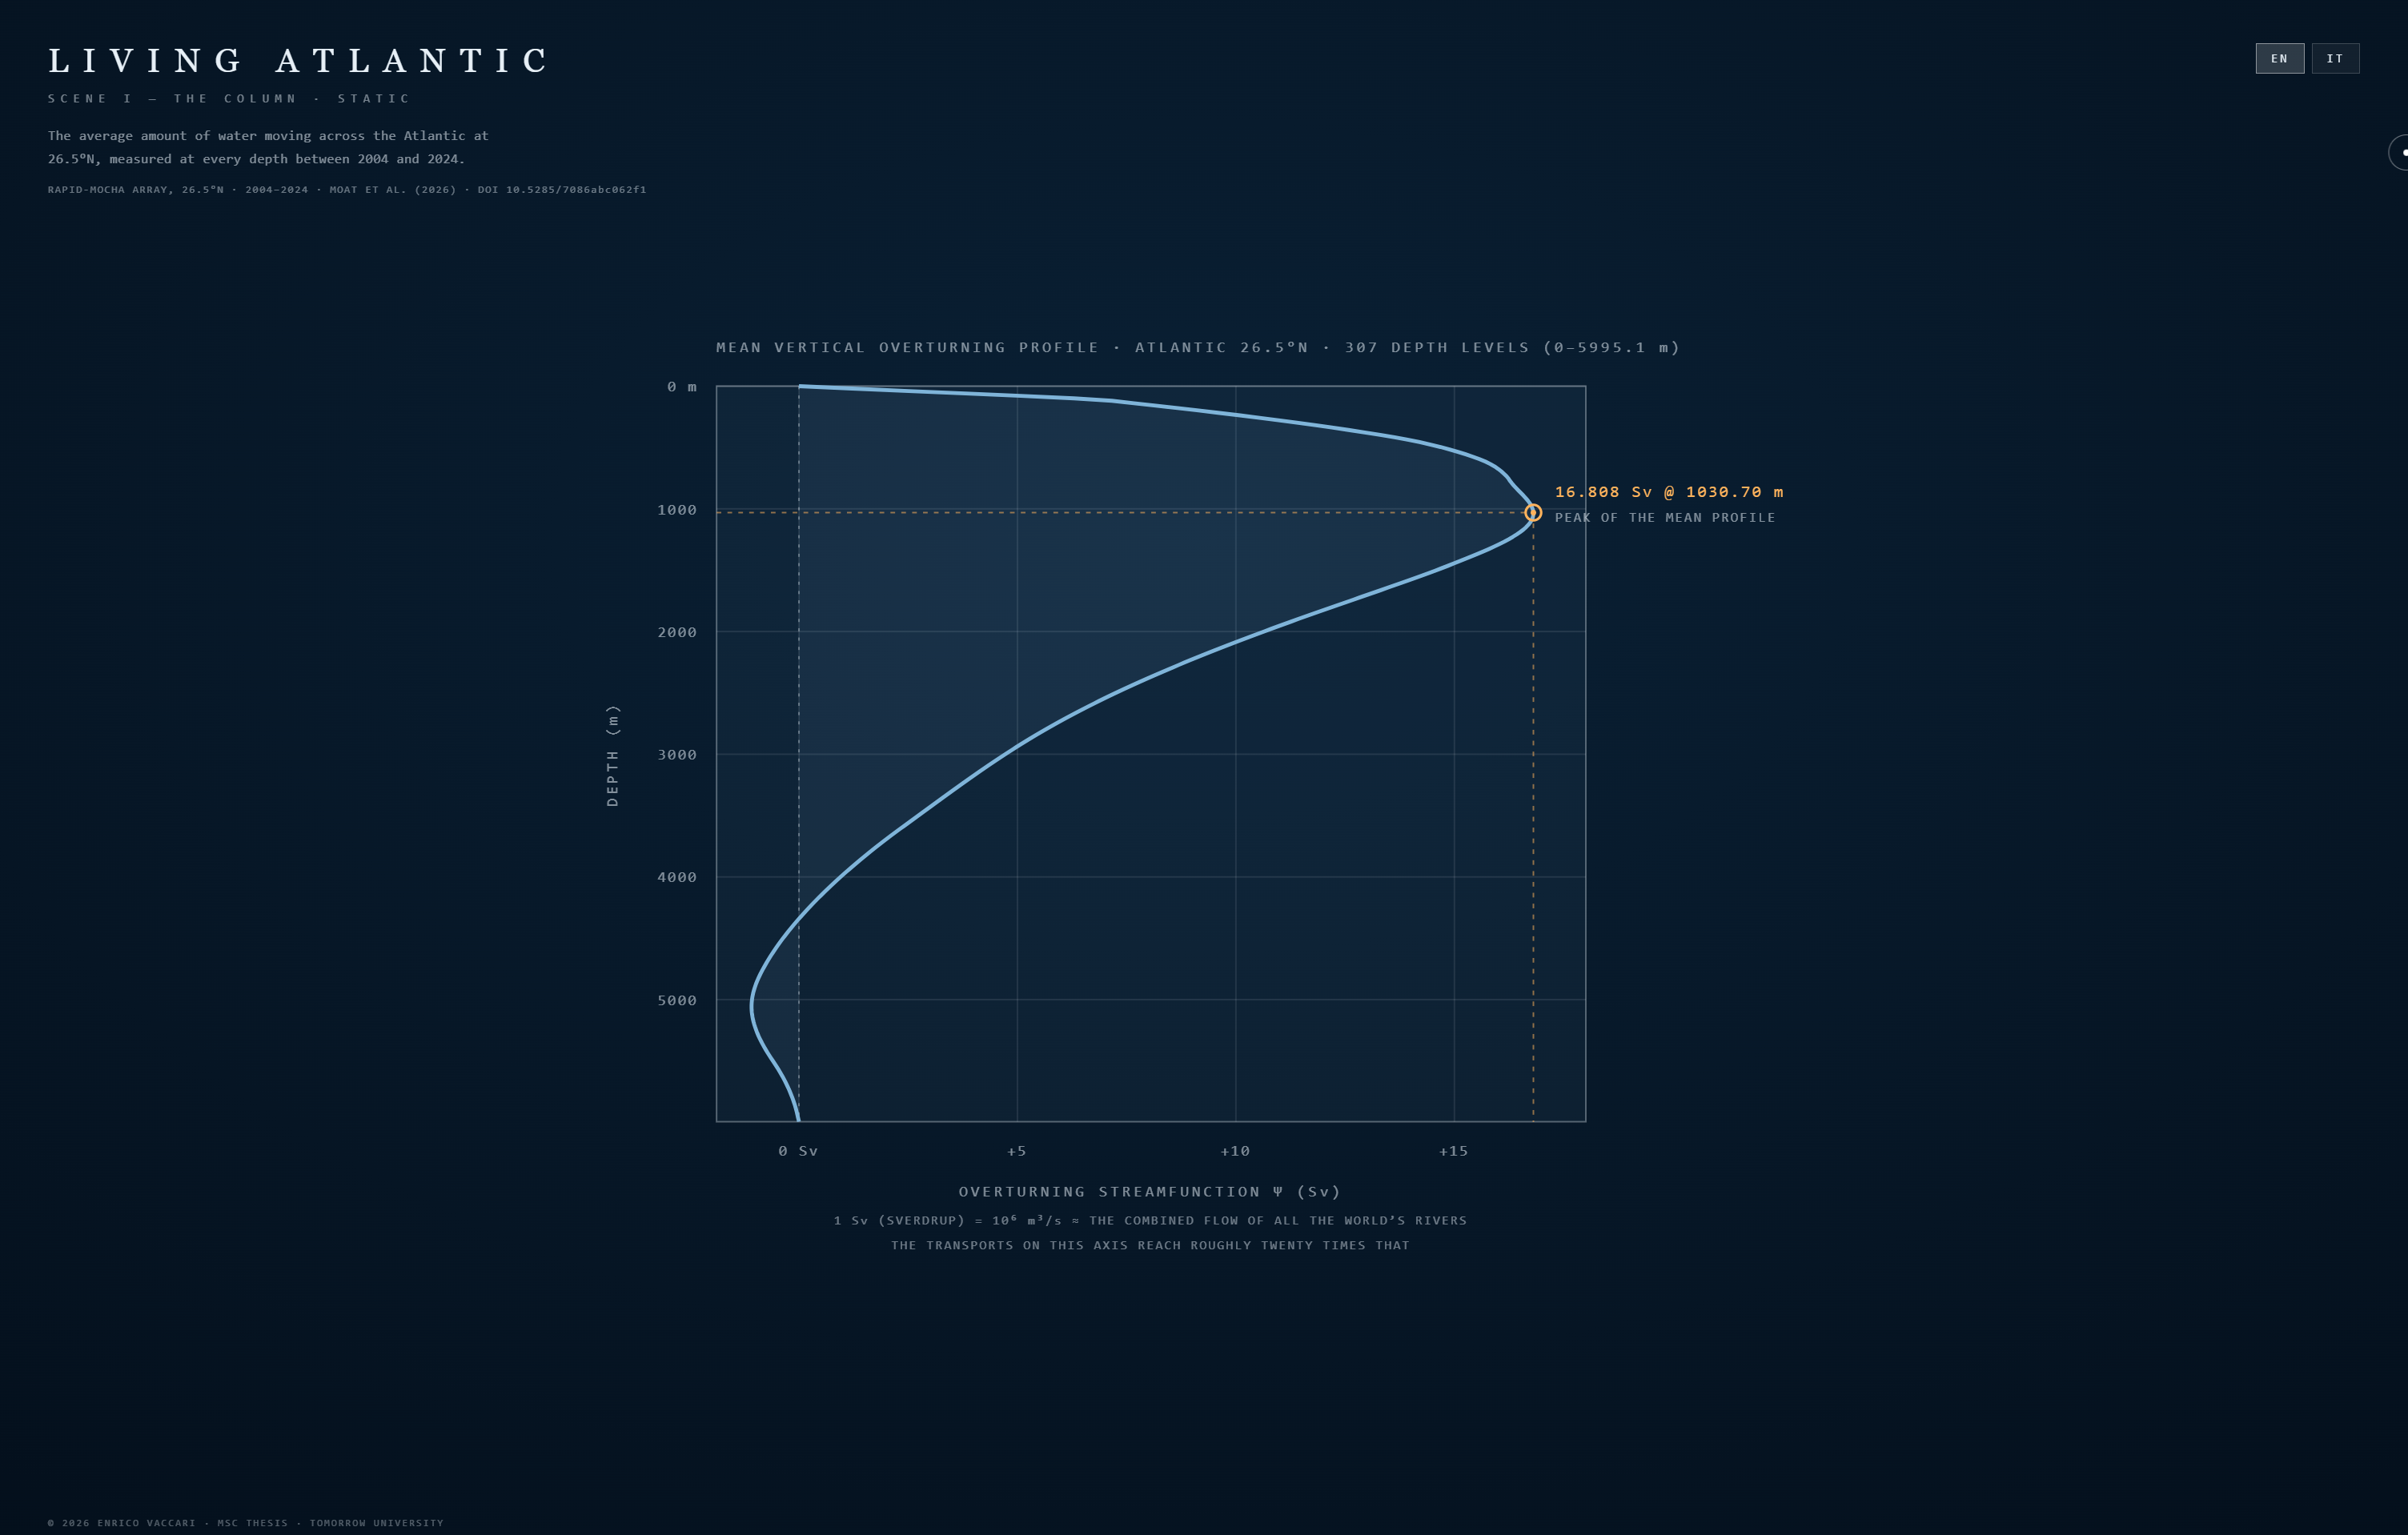
\includegraphics[width=\textwidth]{figures/viz1/viz1_column-static.png}
    \caption{Controllo (C1): il profilo statico canonico.}
    \label{fig:thecolumn-static}
  \end{subfigure}
  \hfill
  \begin{subfigure}[t]{0.48\textwidth}
    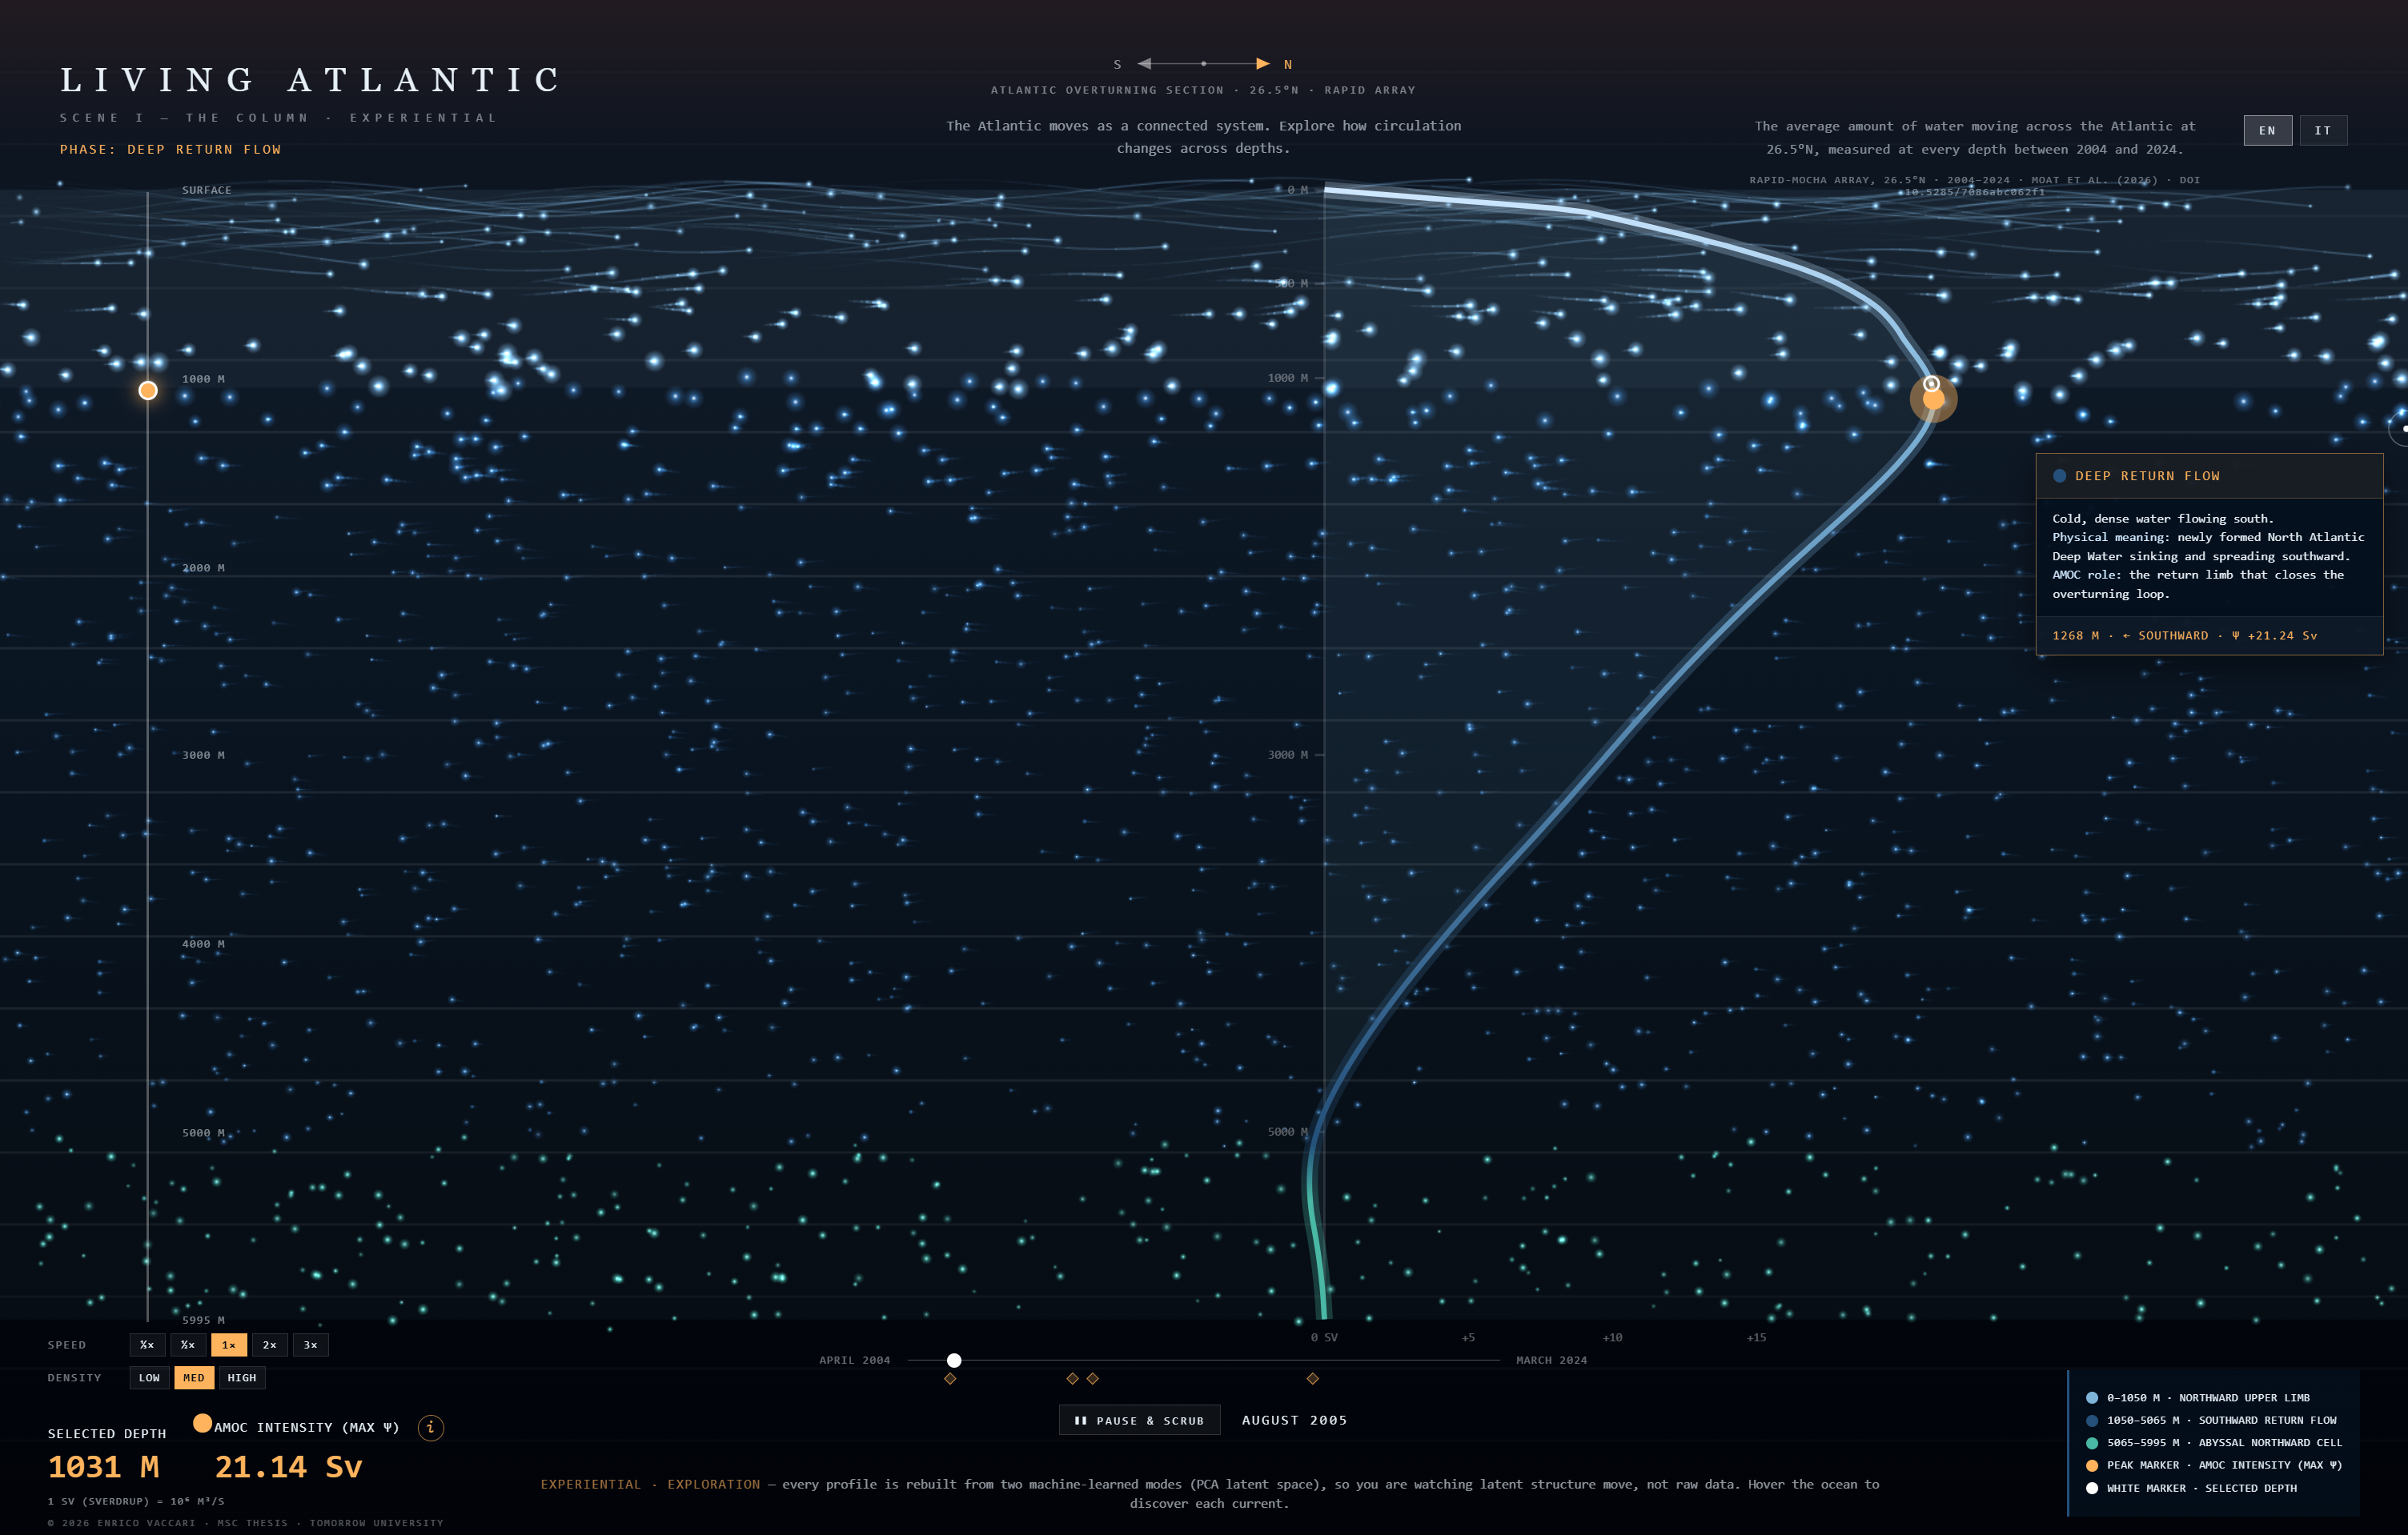
\includegraphics[width=\textwidth]{figures/viz1/viz1_column-experiential.png}
    \caption{Esperienziale (C2+C3): la stessa colonna messa in movimento.}
    \label{fig:thecolumn-experiential}
  \end{subfigure}

  \caption[Le due condizioni della Scena~I]{Le due condizioni somministrate della
  Scena~I, generate dallo stesso bundle di dati attraverso la stessa funzione di
  ricostruzione. La condizione esperienziale introduce il comportamento temporale
  preservando la struttura di fondo della rappresentazione statica.}

  \label{fig:thecolumn-conditions}
\end{figure}


\paragraph{Obiettivo.} Stabilire che l'Atlantico a \ang{26.5}~nord non è una corrente con una posizione ma una quantità distribuita sulla profondità, le cui parti si muovono in direzioni opposte nello stesso momento. Un osservatore che esce sapendo solo che la circolazione è forte o debole non ha ricevuto l'affermazione.

\paragraph{Strategia di rappresentazione.} Il profilo canonico contiene il contro-flusso ma non lo mostra. Per vedere il moto opposto nella curva, un lettore deve sapere che la direzione del flusso a qualsiasi profondità è data dalla \emph{pendenza} della linea anziché dalla sua altezza --- dove la curva sale l'acqua va a nord, dove scende, a sud --- e deve leggere quella pendenza a occhio.

Gli specialisti lo fanno senza accorgersene; i non esperti, come la \S\ref{sec:empirical-viz} ha mostrato, in gran parte no \parencite{harold2016, mcmahon2015, fischer2020}. La Scena~I quindi non aiuta l'osservatore a calcolare la derivata; rende la derivata non necessaria, sostituendo l'inferenza con il movimento.

\paragraph{Mappatura.} L'informazione più importante qui è la struttura verticale (P0), perciò prende la posizione spaziale lungo i 307 livelli di profondità (P1).\footnote{I livelli coprono 0--5995,1\,m e sono quasi uniformemente spaziati, a un intervallo medio di 19,59\,m e un rapporto massimo-minimo di 1,03. La visualizzazione non corregge alcuna non uniformità che non sia nei dati.} Il contro-flusso diventa un campo di particelle avvettato dalla velocità meridionale locale (P2), i mesi anomali diventano disturbo di texture valutato dall'Isolation Forest del Capitolo~\ref{ch:data_pipeline} (P3), e $\mathrm{pc}_1$ guida un impulso sintetizzato, disattivato di default (P5). P4 è assente: la scena mostra una traiettoria e non ha incertezza da codificare. La Tabella~\ref{tab:ledger} registra ciascun elemento rispetto alla sua fonte nel bundle.

Il campo di particelle è guidato dalla derivata, mai da $\Psi$ stessa: guidarlo da $\Psi$ muoverebbe le particelle più velocemente proprio dove la velocità vera è zero, e non potrebbe affatto raffigurare un rovesciamento. I due confini non coincidono e non devono: $\Psi \to 0$ segna dove il trasporto cumulato svanisce (4346,1\,m), mentre $v \to 0$ segna dove il flusso locale si inverte (1050,4\,m e 5065,4\,m).\footnote{Nel profilo medio il picco di 16,808\,Sv sta a 1030,70\,m, con il primo livello diretto a sud immediatamente sotto. Gli ancoraggi di velocità sono riportati alla risoluzione della griglia: la derivazione restituisce il primo livello dove $v$ cambia segno anziché uno zero interpolato. L'attraversamento dello zero di $\Psi$ è riportato in entrambi i modi: 4346,1\,m alla risoluzione della griglia, 4340,85\,m interpolato.}

\paragraph{Condizioni.} C1 è l'idioma canonico: $\Psi$ in funzione della profondità, profondità verso il basso, griglia da pubblicazione, picco segnato, e nient'altro. C2+C3 è la stessa colonna messa in movimento.

C1 non è un confronto indebolito: è tratta dallo stesso bundle attraverso la stessa ricostruzione agli stessi 307 livelli, e il suo marcatore di picco riporta 16,808\,Sv a 1030,70\,m rispetto ai 16,9\,Sv a 1030\,m pubblicati per questo array \parencite{smeed2018}.

\paragraph{Fedeltà.} Ogni profilo in entrambe le condizioni è ricostruito attraverso l'Equazione~\ref{eq:reconstruction}, e l'identità che rende C1 empirica è quella registrata nella \S\ref{subsec:fidelity}.

\paragraph{Dove entra il modello.} Il contributo è duplice. La figura statica è una media di vent'anni, e le medie non si muovono; $\mathrm{pc}_1$ e $\mathrm{pc}_2$ rendono ogni mese un punto, così che camminare tra i punti ricostruisca ogni mese a sua volta. Il movimento non è quindi un'animazione aggiunta a una figura ma il modello che percorre la sua traiettoria appresa, con H2 che rende quel percorso fedele anziché comodo. Il modello segnala anche quali mesi si discostano dal record, che diventano texture; tutto il resto --- campo di particelle, assi, lettura del picco --- è classico.

\paragraph{Contributo atteso.} C1 mostra dove l'Atlantico è forte in media. C2 mostra ciò che C1 contiene ma non può mostrare. C3 aggiunge il tempo che il modello ha appreso: la colonna si gonfia verso 24,26\,Sv a gennaio~2018 e collassa verso 5,71\,Sv a marzo~2013, circa $3.5\sigma$ sotto la media dei massimi mensili, e il picco migra mentre procede --- 1070,2\,m nel mese più forte, 991,1\,m nel più debole.
\footnote{La migrazione è il secondo modo all'opera: $\mathrm{pc}_1$ fissa quanta acqua la colonna trasporta, $\mathrm{pc}_2$ la ridistribuisce verticalmente. Una bozza precedente di questa tesi affermava che la profondità del trasporto massimo è stabile mentre la sua entità varia; valutato lungo il record, non è così.} L'affermazione non è che la condizione esperienziale sia più attraente, ma che ciò che l'idioma statico non riesce a trasmettere --- struttura che va inferita, cambiamento che va immaginato --- è ciò che il movimento e il tempo latente consegnano direttamente.

\subsection{Scena II: La sala macchine}
\label{subsec:scene-engine}

\begin{quote}
\textbf{Domanda guida.} \emph{Guardando l'oceano muoversi da stato a stato nel tempo, va sempre da qualche parte di nuovo, oppure a volte ripassa per dove è già stato?}
\end{quote}

\begin{figure}[htbp]
  \centering

  \begin{subfigure}[t]{0.48\textwidth}
    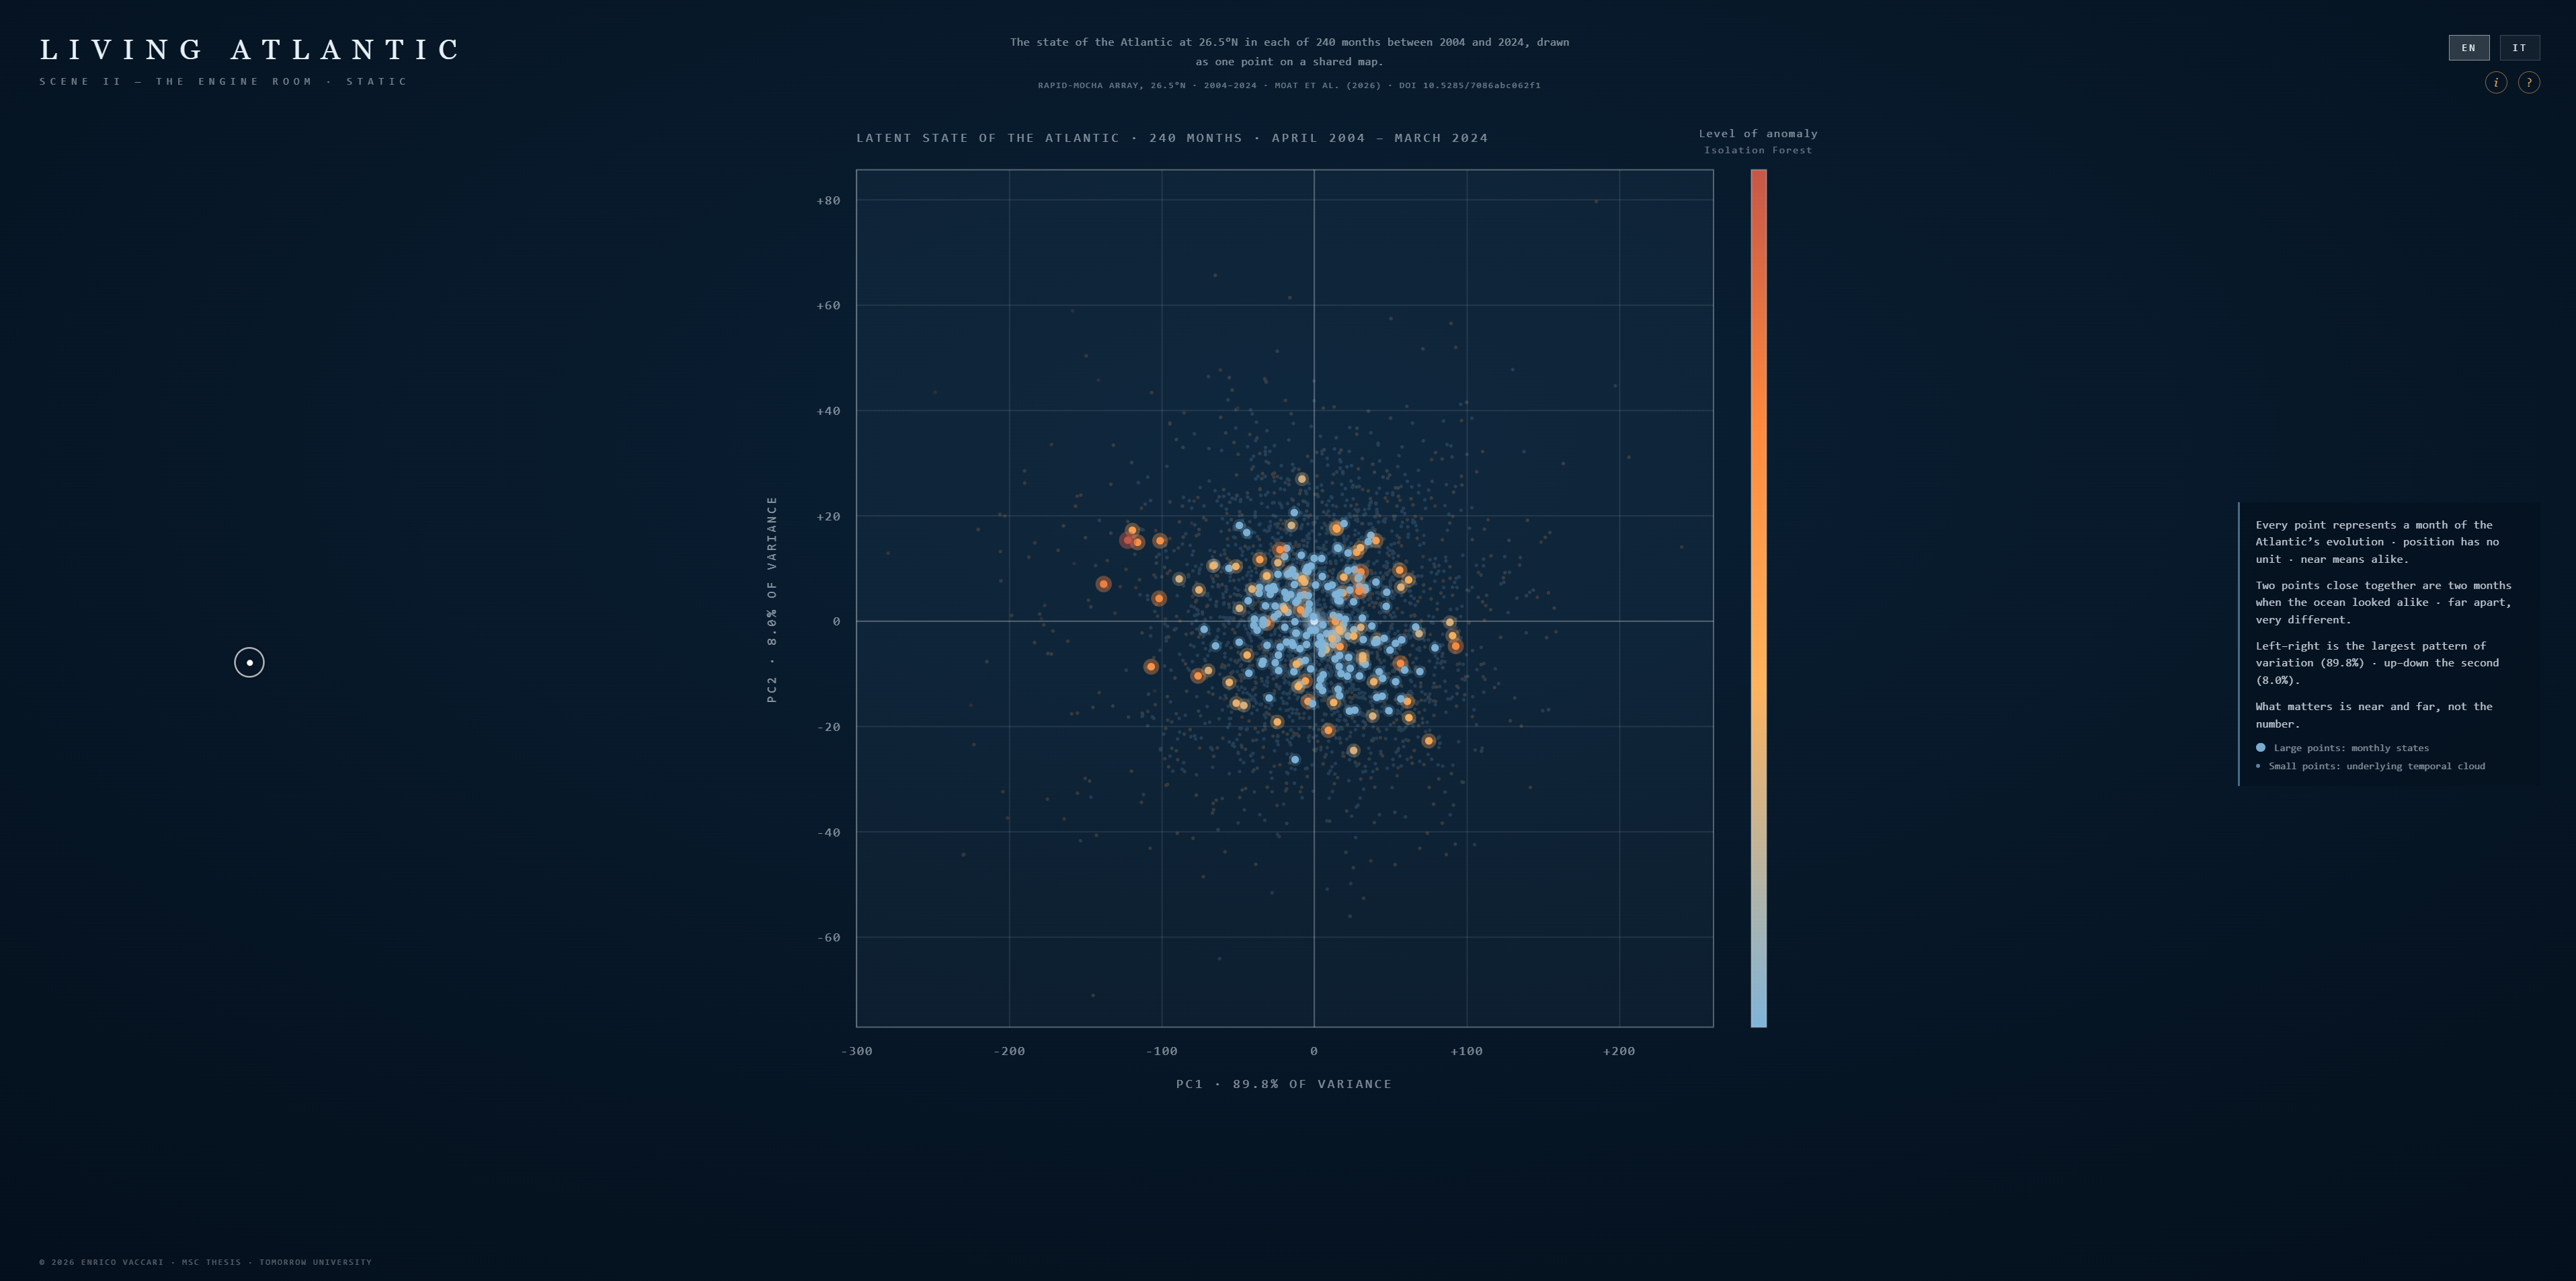
\includegraphics[width=\textwidth]{figures/viz2/viz2_theengine-static.png}
    \caption{Controllo (C1): la rappresentazione statica dello spazio latente.}
    \label{fig:theengine-static}
  \end{subfigure}
  \hfill
  \begin{subfigure}[t]{0.48\textwidth}
    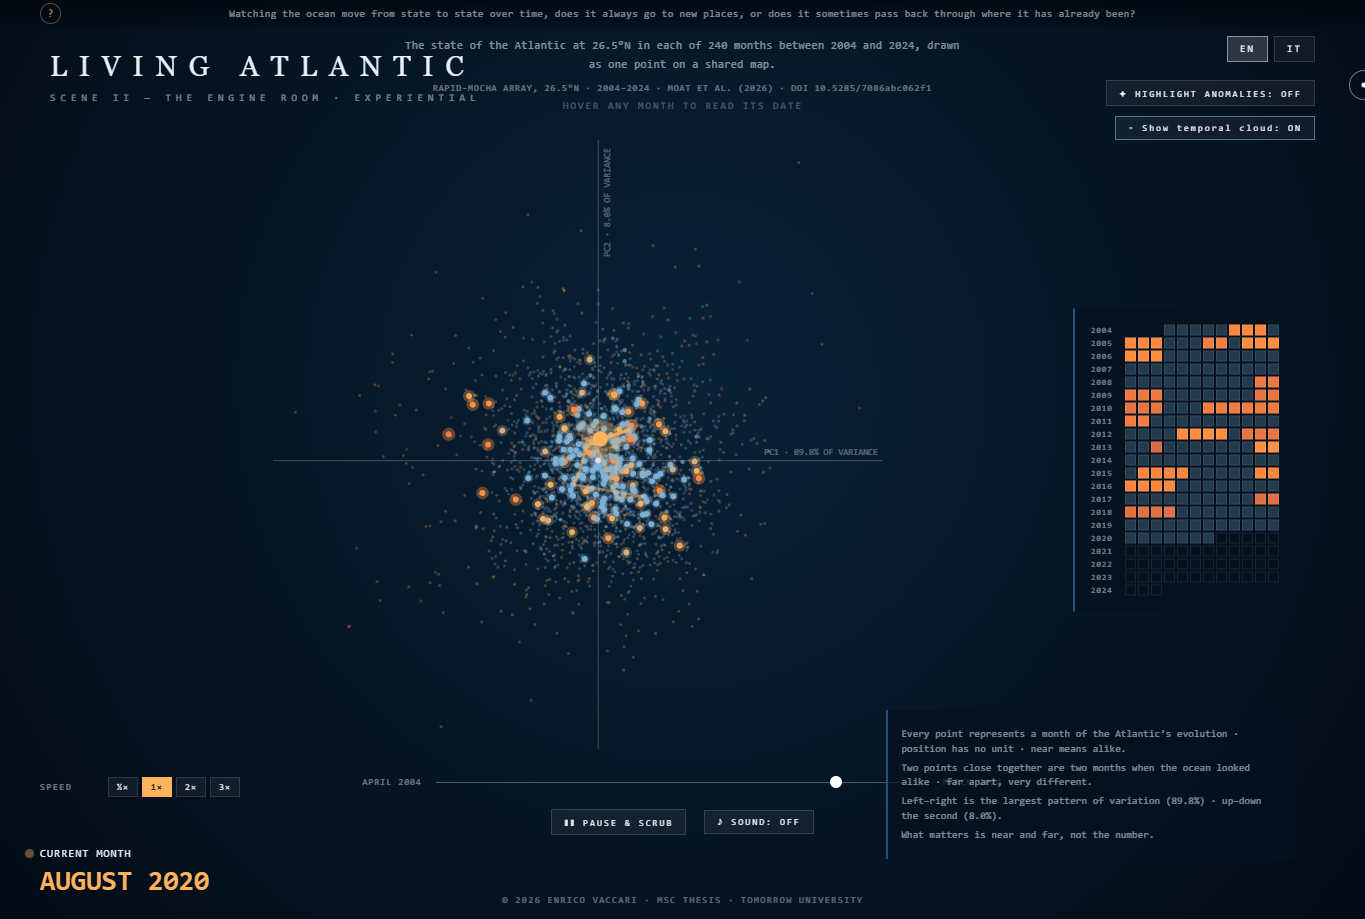
\includegraphics[width=\textwidth]{figures/viz2/viz2_theengine-experiential.png}
    \caption{Esperienziale (C2+C3): la traiettoria in evoluzione attraverso lo spazio latente.}
    \label{fig:theengine-experiential}
  \end{subfigure}

  \caption[Le due condizioni della Scena~II]{Le due condizioni somministrate della
  Scena~II, tratte dalle stesse coordinate latenti nel bundle di dati. La condizione
  statica mostra gli stati mensili come uno scatter fisso; la condizione esperienziale
  percorre gli stessi stati nel tempo.}

  \label{fig:theengine-conditions}
\end{figure}


\paragraph{Obiettivo.} Rendere il piano latente del Capitolo~\ref{ch:data_pipeline} uno spazio abitabile anziché uno strumento d'analista. Ogni mese del record è un punto, e la prossimità significa somiglianza. L'affermazione che la scena deve consegnare è che il sistema, lasciato vagare, ritorna: ripassa per stati che ha già occupato.\footnote{Questa ricorrenza caratterizza le dinamiche del presente record osservativo, in cui l'AMOC oscilla entro un regime stabile plasmato dal forzante stagionale e dalla variabilità interna. Non è evidenza che il sistema non possa subire transizioni di lungo periodo.}

\paragraph{Strategia di rappresentazione.} Il modo canonico di mostrare uno spazio latente è uno scatter di punti colorati per tempo \parencite{sacha2018}. Quella figura contiene la ricorrenza ma non può mostrarla: due punti possono stare quasi uno sull'altro pur distando anni, e una nuvola statica non dà all'occhio alcun modo di sapere che il percorso ha lasciato l'uno ed è poi arrivato all'altro. La ricorrenza è una proprietà della traiettoria, non dell'insieme di punti. La Scena~II percorre quindi il cammino nel tempo e accumula gli stati visitati come una nuvola.

\paragraph{Mappatura.} Ogni mese prende una posizione nel piano $\mathrm{pc}_1 \times \mathrm{pc}_2$, con gli assi etichettati con la varianza che ciascun modo spiega (P1). Il tempo diventa movimento reale lungo il percorso, e l'entità del cambiamento da mese a mese diventa la violenza visibile di ciascun passo (P2): i passi più grandi sono quattro volte la mediana, e quella variazione è segnale anziché rumore da lisciare.\footnote{I tre passi più grandi cadono su mesi che la fase di rilevamento segnala indipendentemente come anomali --- una coerenza interna registrata nell'Appendice~\ref{app:code}, non un'affermazione fatta a schermo.} I mesi anomali agitano il marcatore (P3) e $\mathrm{pc}_1$ guida il suono (P5); P4 è di nuovo assente.

\paragraph{Condizioni.} C1 è lo scatter canonico: i 240 mesi nel piano, colorati per livello di anomalia --- il punteggio Isolation Forest di ciascun mese, come registra la barra dei colori --- statico, non annotato e privo di ogni ordinamento nel tempo, così che un osservatore non abbia nulla con cui tracciare un ritorno. C2+C3 sono gli stessi punti, dati e colori, messi in movimento. Entrambe le condizioni mostrano la stessa nuvola sub-mensile più fine dietro i punti mensili, così che un mese si legga come la media di uno sciame inquieto anziché come un singolo stato.\footnote{Da \texttt{manifold\_cloud} nel bundle. La colorazione di anomalia è presa dal punteggio Isolation Forest del mese di ciascun punto, non dalla distanza dal centroide della nuvola; un surrogato spaziale codificherebbe ``lontano dal centro'' come ``raro'', che è parte della lettura che la scena deve trattenere.} Nessuna delle due condizioni disegna il profilo ricostruito: collegare il piano alla colonna darebbe al gruppo sperimentale informazione che il controllo non ha.

\paragraph{Fedeltà.} Il segno di ciascuna componente principale è arbitrario, perciò entrambe le condizioni rendono il piano con orientamento identico --- la nuvola che un partecipante di controllo vede è la stessa nuvola, non la sua immagine speculare --- e unità uguali su entrambi gli assi mantengono la distanza a schermo uguale alla distanza nello spazio latente.

\paragraph{Dove entra il modello.} Qui il modello non è substrato ma terreno. Il piano non esiste in natura: è la base che la decomposizione ha trovato, e ogni posizione in esso è una proiezione appresa. La Scena~I usava le coordinate latenti per animare un oggetto fisico; la Scena~II rende il sistema di coordinate stesso l'oggetto dell'attenzione, che è il passo dall'analisi esperta alla comunicazione pubblica che la \S\ref{sec:translate-premise} rivendica. La ricorrenza che un partecipante cerca è una proprietà di quello spazio appreso, percepibile solo perché H2 ha stabilito che lo spazio è abbastanza piatto da essere percorso senza distorsione. A differenza della Scena~I, nulla qui esisterebbe senza il modello.

\paragraph{Contributo atteso.} Lo scatter statico mostra che l'Atlantico occupa un insieme limitato di stati; la condizione esperienziale mostra ciò che esso contiene ma non può mostrare --- che il sistema si muove attraverso quell'insieme con struttura, alla deriva in certi momenti e a scatti in altri, e che ritorna.

\subsection{Scena III: La soglia}
\label{subsec:scene-threshold}

\begin{quote}
\textbf{Domanda guida.} \emph{Pensi che quanto i modelli concordano tra loro sia rimasto lo stesso in tutti gli anni, o sia cambiato?}
\end{quote}

\begin{figure}[htbp]
  \centering

  \begin{subfigure}[t]{0.48\textwidth}
    \vspace{0pt}
    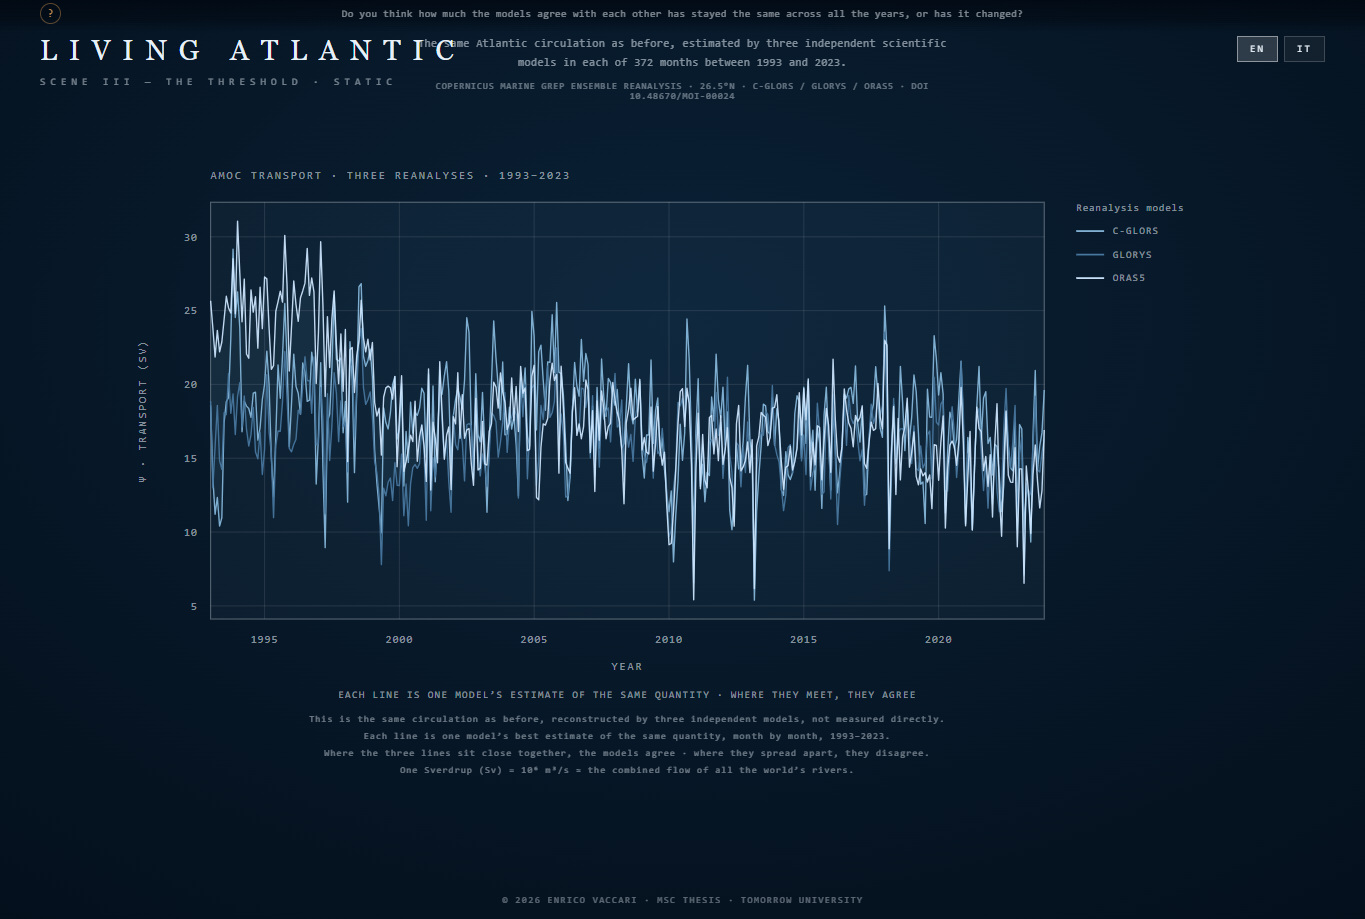
\includegraphics[width=\textwidth]{figures/viz3/viz3_thethreshold-static.png}
    \caption{Controllo (C1): le tre serie di rianalisi, statiche.}
    \label{fig:thethreshold-static}
  \end{subfigure}
  \hfill
  \begin{subfigure}[t]{0.48\textwidth}
    \vspace{0pt}
    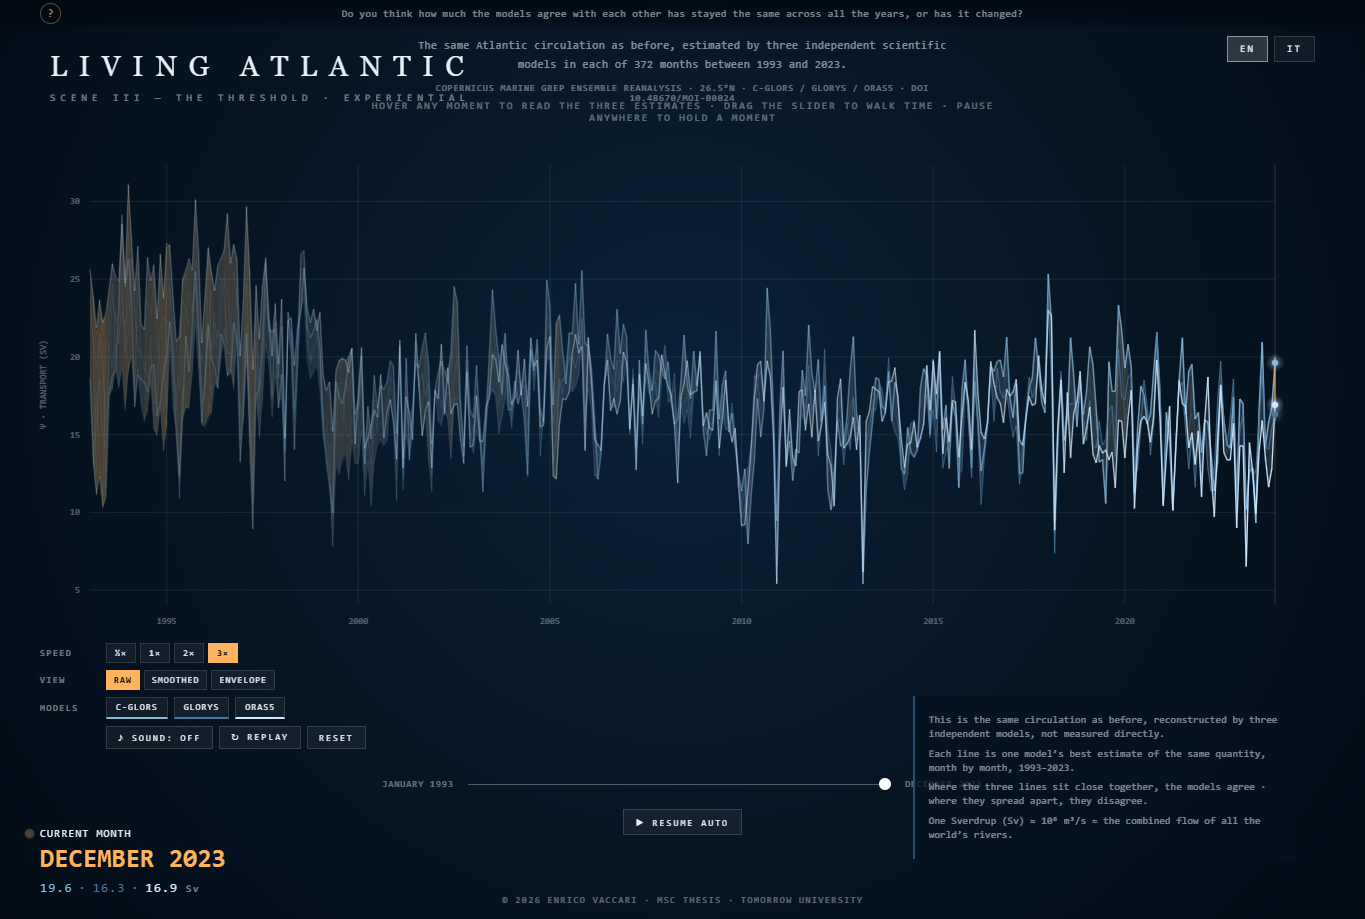
\includegraphics[width=\textwidth]{figures/viz3/viz3_thethreshold-experiential.png}
    \caption{Esperienziale (C2+C3): le stesse serie, con il loro disaccordo reso come movimento.}
    \label{fig:thethreshold-experiential}
  \end{subfigure}

  \caption[Le due condizioni della Scena~III]{Le due condizioni somministrate della
  Scena~III, tratte dagli stessi tre membri di rianalisi Copernicus. La condizione
  statica mostra le tre serie tutte insieme; la condizione esperienziale rende il loro
  disaccordo mutevole come movimento e suono.}

  \label{fig:thethreshold-conditions}
\end{figure}


\paragraph{Obiettivo.} Rendere l'incertezza una qualità sentita anziché un numero. Le Scene~I e~II mostravano una quantità misurata da un array nell'acqua; la Scena~III mostra la stessa quantità ricostruita in tre modi diversi, da tre rianalisi oceaniche che concordano nel presente e divergono nel passato.\footnote{Rianalisi d'ensemble Copernicus Marine GREP, membri C-GLORS, GLORYS e ORAS5, mensile da gennaio~1993 a dicembre~2023.}

\paragraph{Strategia di rappresentazione.} L'idioma canonico traccia l'ensemble come una media con una banda ombreggiata, o come linee dei membri sovrapposte. Entrambi contengono il mutevole disaccordo ma lo presentano come una distanza da misurare tra le curve --- il compito inferenziale che la Scena~I si propone di rimuovere. La Scena~III rende invece il disaccordo una proprietà del medium: dove le ricostruzioni convergono il display è calmo, dove divergono diventa visibilmente e udibilmente agitato. Questo realizza P4, tenuto in riserva per le prime due scene, e con esso DP2.2: il mutevole disaccordo è reso come variazione percettiva anziché come annotazione numerica.

\paragraph{Mappatura.} La quantità più importante qui non è il valore di trasporto ma il mutevole disaccordo, perciò prende il canale più forte e diventa movimento (P0). La stima di ciascun membro tiene una posizione nel tempo (P1), che a sua volta diventa movimento reale (P2). L'incertezza diventa variabilità animata (P4): turbolenza, larghezza della banda e temperatura di colore scalano tutte con la dispersione reale tra i membri a ciascun mese, e nessuna è mai stampata come numero. La stessa dispersione guida una texture audio, pulita quando i modelli concordano e che si fa ruvida mentre si separano (P5). P3 è assente, non essendo l'anomalia centrale all'affermazione.

\paragraph{Condizioni.} C1 disegna le tre linee dei membri nel tempo, distinguibili e nominate, statiche e non annotate: nessuna epoca è ombreggiata, nessun anno segnato. C2+C3 mette le stesse linee in movimento e aggiunge il medium vivente tra esse, con controlli che permettono a un osservatore di rivedere dati identici a diverse aggregazioni --- grezzi, lisciati su una finestra scelta, o il solo inviluppo --- e isolare una qualsiasi singola rianalisi.\footnote{Queste sono viste di un unico dataset, non informazione aggiuntiva: ogni aggregazione è calcolata dalle stesse tre serie dei membri, e i valori grezzi restano disponibili in entrambe le condizioni.}

\paragraph{Fedeltà.} Ogni proprietà visiva e uditiva è guidata dalla dispersione reale tra i tre membri a ciascun mese, e nessuna aggregazione introduce una quantità che i membri non contengono. Le tre linee non sono mai ridotte a una media con barre d'errore: il soggetto della scena sono tre ricostruzioni in disaccordo, non una stima con un margine.

\paragraph{Dove entra il modello.} Meno delle tre, e l'asimmetria è istruttiva. Le tre rianalisi sono modelli oceanici fisici prodotti da altre istituzioni, non rappresentazioni apprese costruite per questa tesi, e la dispersione tra esse è aritmetica: il contributo di machine learning del Capitolo~\ref{ch:data_pipeline} non guida questa scena. Ciò che si trasferisce è la grammatica anziché il modello --- gli stessi principi che mappavano la struttura latente sul movimento nelle Scene~I e~II qui mappano il disaccordo d'ensemble su variabilità animata, senza uno spazio latente su cui poggiare. Che la grammatica sopravviva alla rimozione del modello è l'evidenza più forte disponibile entro questa tesi per l'obiettivo~O2.2.

\paragraph{Contributo atteso.} Il grafico statico mostra che tre modelli stimano la stessa quantità e non concordano del tutto; la condizione esperienziale mostra che il grado di accordo è esso stesso una variabile --- le ricostruzioni che si separano nel record più antico e convergono man mano che il vincolo osservativo migliora, con la dispersione media che si dimezza all'incirca tra il decennio pre-2004 e gli anni dell'array.\footnote{Il restringimento è graduale anziché un gradino all'installazione dell'array, e l'artefatto non segna alcuna data; il cambiamento è lasciato da percepire anziché annunciato.} Se un non specialista legga quel cambiamento come un cambiamento di certezza --- anziché come una variazione decorativa --- è ciò che l'aspettativa~E3.2 verifica.

% ============================================================
% Tabella riassuntiva
% ============================================================
\begin{table}[tbp]
\centering
\caption[Le tre scene a colpo d'occhio]{Le tre scene di \emph{Living Atlantic}: la domanda che ciascuna pone all'osservatore, i principi che realizza, e ciò che il machine learning contribuisce. Il contributo diminuisce lungo la discesa --- e la sopravvivenza della grammatica fino alla Scena~III, dove nessun modello appreso guida il display, è l'evidenza della sua trasferibilità (O2.2).}
\label{tab:scene-summary}
\small
\renewcommand{\arraystretch}{1.35}

\begin{tabularx}{\textwidth}{@{}p{2.6cm} X p{2.5cm} X@{}}
\toprule
\textbf{Scena} &
\textbf{Domanda guida} &
\textbf{Principi} &
\textbf{Cosa aggiunge il ML} \\
\midrule

\makecell[l]{Scena I\\La colonna} &
L'acqua si muove tutta allo stesso modo; se no, in quali direzioni? &
P0, P1, P2, P3, P5 &
Le coordinate latenti lungo cui il profilo si muove, e i punteggi di anomalia che ne disturbano la texture. Il campo di particelle è classico. \\

\makecell[l]{Scena II\\La sala macchine} &
L'oceano va sempre verso qualcosa di nuovo, o ripassa per dove è già stato? &
P1, P2, P3, P5 &
Il piano stesso: lo spazio percorso è la base appresa. Nulla nella scena esiste senza il modello. \\

\makecell[l]{Scena III\\La soglia} &
L'accordo tra i modelli è rimasto lo stesso negli anni, o è cambiato? &
P0, P1, P2, P4, P5 &
Il minore dei tre. Le rianalisi sono modelli fisici esterni; la grammatica porta la scena senza uno spazio appreso. \\

\bottomrule
\end{tabularx}
\end{table}
